
\chapter{Ethereum}

\section{Legacy Ethereum (Ethereum 1.0)}

\subsection{Recursive Length Prefix (RLP) encoding}
Recursive Length Prefix (RLP) serialization is used extensively in Ethereum's execution clients. RLP standardizes the transfer of data between nodes in a space-efficient format. The purpose of RLP is to encode arbitrarily nested arrays of binary data, and RLP is the primary encoding method used to serialize objects in Ethereum's execution layer.

RLP does not deal with strings, and other "types" and delegates the encoding of those to the underlying binary data to some higher-order protocols. RLP only deals with binary blobs and positive integers.

\begin{figure}[h]
    \centering
    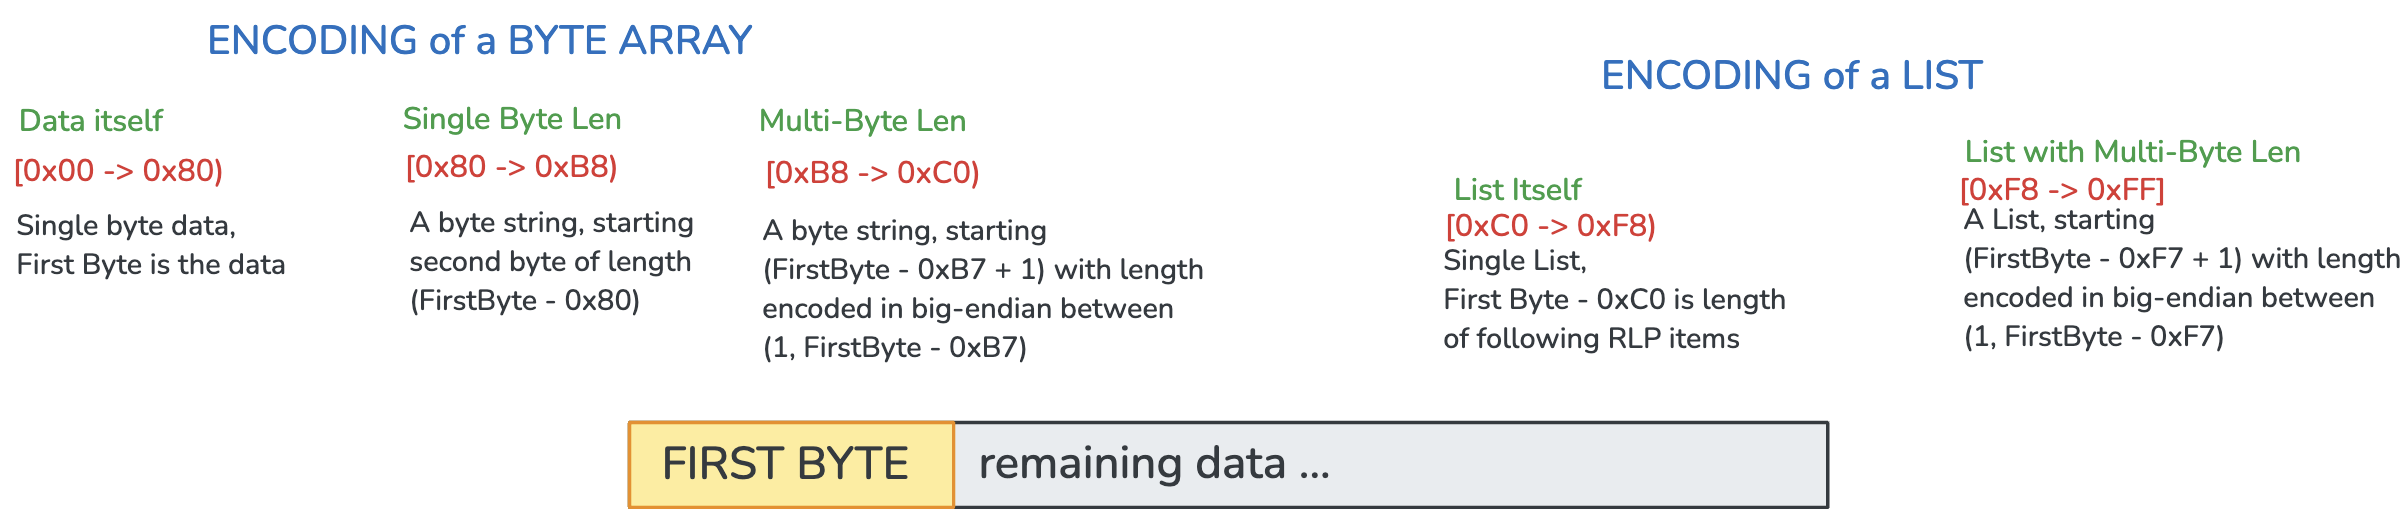
\includegraphics[width=1.0\textwidth]{ethereum/assets/rlp-encoding-first-byte.png}
    \caption{The first byte of an RLP serialized blob describes how to parse data.}
    \label{fig:first-byte-rlp}
\end{figure}

RLP only deals with "items". Essentially:
\begin{itemize}
    \item A "byte array" is an item.
    \item A positive integer is an item. Essentially, this is also converted into a "byte array" by converting it to a smallest possible big-endian representation of the integer.
    \item A list of items is an item.
\end{itemize}

The first byte of an RLP serialized blob is a "type" byte \footnote{RLP on ethereum.org: \href{https://ethereum.org/en/developers/docs/data-structures-and-encoding/rlp/}{https://ethereum.org/en/developers/docs/data-structures-and-encoding/rlp/}}. See figure \ref{fig:first-byte-rlp} for the description.

\subsection{How to deploy a contract: \code{CREATE} vs \code{CREATE2}}
Deploying a contract on Ethereum involves creating a new contract instance and assigning it an address. The creation part is done via creating an instance of \code{init\_code}, which is a constructor code which when executed under an EVM call frame, generates the bytecode of the contract. The simplest instance would be a "default constructor" where the \code{init\_code} just returns the required bytecode verbatim.

As far as assignment of the address goes, how that address is assigned depends on the method of deployment. There are two methods of deploying a contract:
\begin{itemize}
    \item \code{CREATE}: This is the original method of deploying a contract. The address is determined by the sender's address and the nonce (number of transactions sent from that address). The address is calculated as:
    \[
    \text{address} = \text{keccak256}(\text{rlp}(\text{sender}, \text{nonce}))\text{[12:]}
    \]
    where \text{rlp} is the recursive length prefix encoding.
    
    \item \code{CREATE2}: Introduced in \href{https://eips.ethereum.org/EIPS/eip-1014}{EIP-1014}, this method allows for more flexibility in determining the address. The address is calculated using the sender's address, a salt value, and the bytecode of the contract. The address is calculated using the last 20 bytes of the keccak256 hash of the following:
    \[
    \text{address} = \text{keccak256}(\text{0xff}, \text{sender}, \text{salt}, \text{keccak256(initCode)})\text{[12:]}
    \]
\end{itemize}

\subsubsection{Addresses generated by \code{CREATE2} seldom collide with addresses generated via \code{CREATE}}
It is guaranteed that the address will not collide with addresses generated via \code{CREATE} as the \code{0xff} RLP prefix is used only for data that is petabytes long. This is because if we compare \code{rlp(...)} to \code{0xff + ...}, the \code{rlp(...)} will seldom have a \code{0xff} prefix, especially if it is as in \code{CREATE} opcode (\code{rlp(sender, nonce)} is too small as compared to patabytes of data that will allow the first byte of RLP encoding to be \code{0xff}).

\subsubsection{Address collision between \code{CREATE} and \code{CREATE2}}
There still is a small possibility that the address generated by \code{CREATE2} will collide with an address generated by \code{CREATE}. When that happens, upon execution, an assert is done which checks that the destination address has any non-zero nonce, and non-zero code. In case that is true, a revert is thrown.

\subsection{Wintermute Hack (2022): \code{CREATE} and EIP-155 for transaction signatures}
\href{https://www.wintermute.com/}{Wintermute} was engaged by the Optimism Foundation for liquidity provisioning services on the \$OP launch. On May 27, 2022, 20 million \$OP was allocated to Wintermute from the Foundation's Partner Fund. However, Wintermute later found that they could not access these tokens because they had provided an Ethereum (L1) multisig address that they had not yet deployed to Optimism (L2), where the allocated funds were sent. Unfortunately, an attacker found this and deploy the multisig contract with the same address to L2 before Wintermute, effectively gaining control over the funds.

Wintermute also later put out a message to optimism community \footnote{Wintermute message: \href{https://gov.optimism.io/t/message-to-optimism-community-from-wintermute/2595}{https://gov.optimism.io/t/message-to-optimism-community-from-wintermute/2595}}.

To understand this hack better, let's enumerate the important addresses concerned \footnote{A complete stepwise description of hack has been borrowed from \href{https://inspexco.medium.com/how-20-million-op-was-stolen-from-the-multisig-wallet-not-yet-owned-by-wintermute-3f6c75db740a}{https://inspexco.medium.com/how-20-million-op-was-stolen-from-the-multisig-wallet-not-yet-owned-by-wintermute-3f6c75db740a}}:
\begin{enumerate}
    \item \textbf{MultiSig address}(0x4f..81): The address $\text{0x4f3a120e72c76c22ae802d129f599bfdbc31cb81}$ where funds from Optimism Foundation were received on the Optimism chain (Chain ID = 10). This address on Ethereum (Chain ID = 1) hosted a Gnosis Safe Multisig wallet and was controlled fully by Wintermute. This wallet however was not deployed on the Optimism chain and was an unused address.
    \item \textbf{Gnosis Safe Proxy Factory}(0x76..9b): The address $\text{0x76e2cfc1f5fa8f6a5b3fc4c8f4788f0116861f9b}$ is the Gnosis Safe Proxy Factory contract deployed on Ethereum, but was not deployed on Optimism. This contract is used to create Gnosis Safe wallets, the MultiSig wallet $\text{0x4f..81}$ above. This contract used \code{new} keyword to create the wallet, which uses \code{CREATE} opcode under the hood.
    \item \textbf{Gnosis Safe Proxy Deployer}(0x1a..6a): The address $\text{0x1aa7451dd11b8cb16ac089ed7fe05efa00100a6a}$ is the EOA (Externally Owned Account) that deployed the Gnosis Safe Proxy Factory contract on Ethereum. This address did not exist on Optimism however. Since it also used \code{CREATE} opcode, only it can reliably deploy the same address on Optimism. The attacker did not know the private key behind this EOA, which is a secret that only Gnosis Safe team holds.
\end{enumerate}

\subsubsection{Description of the hack}
The hack made use of two vulnerabilities:
\begin{itemize}
    \item Use of the \code{CREATE} opcode.
    \item Use of non-chain specific transaction signatures introduced in EIP-155.
\end{itemize}
The following figure \ref{fig:wintermute-hack} shows the steps of the hack.

\begin{figure}[h]
    \centering
    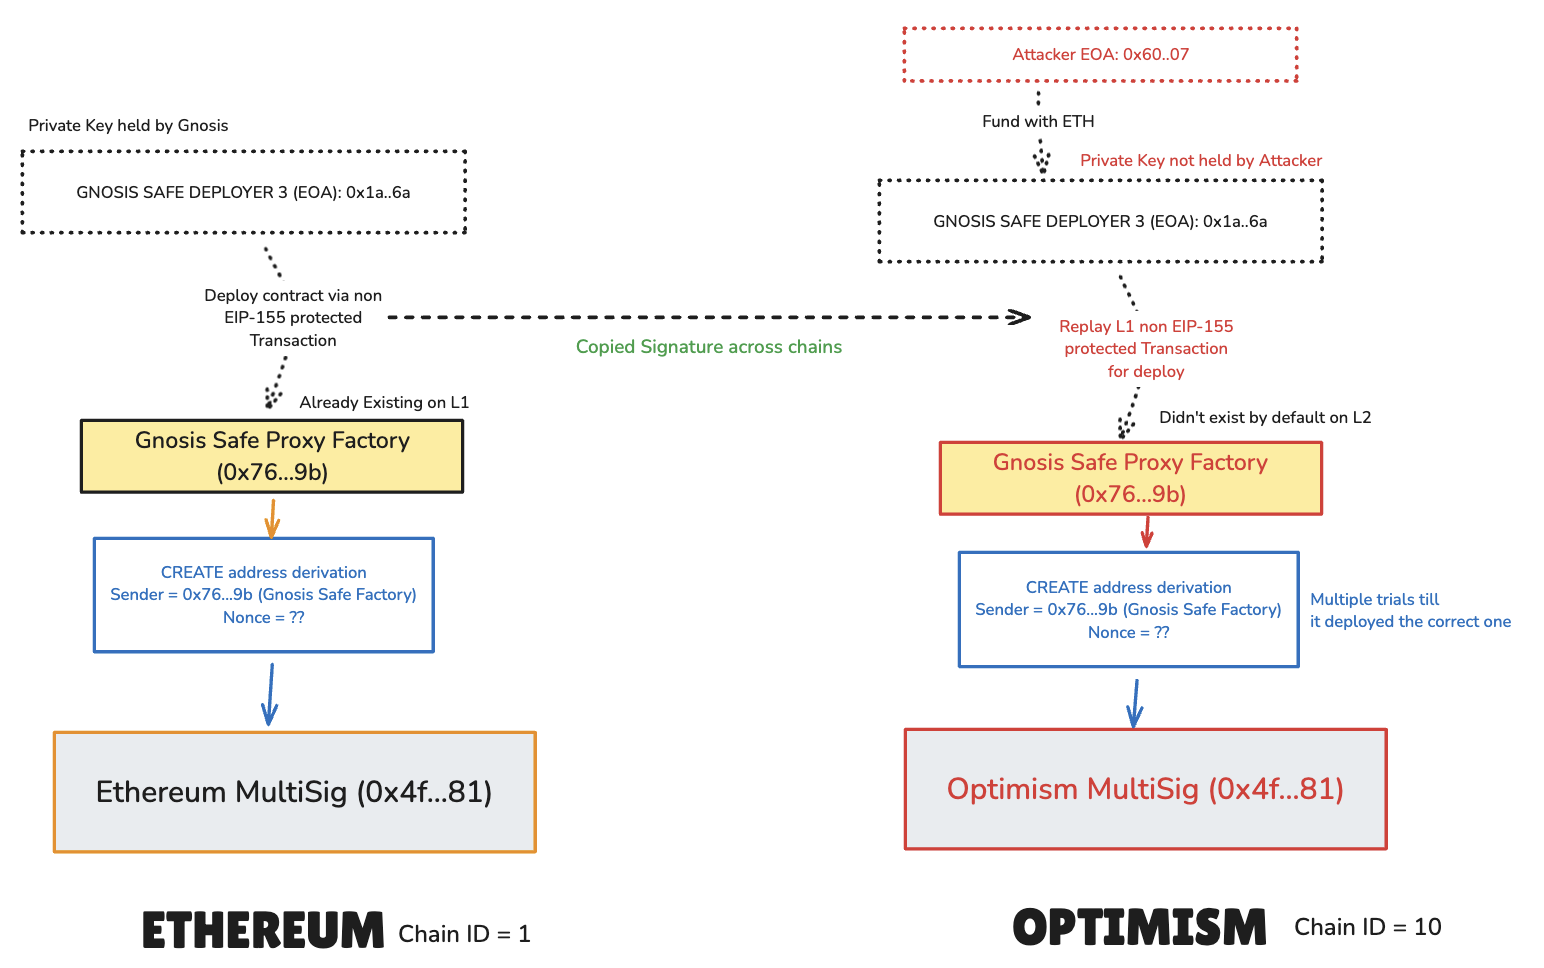
\includegraphics[width=1.0\textwidth]{ethereum/assets/wintermute-hack.png}
    \caption{The steps of the Wintermute hack (2022).}
    \label{fig:wintermute-hack}
\end{figure}

\begin{Exercise}[title={Ethereum Deployments}]
    \begin{enumerate}
        \item Explain in detail the difference between \code{CREATE} and \code{CREATE2} in terms of how they generate addresses for deployed contracts. Why is \texttt{0xFF} prefix added when calculating the hash in \code{CREATE2}?
    \end{enumerate}
\end{Exercise}
\begin{Answer}
    \begin{enumerate}
        \item \todo{Add an answer here}
    \end{enumerate}
\end{Answer}

\subimport{./}{eip-2935.tex}
\section{Ethereum after Merge (Ethereum 2.0)}
\todo{Introduce SSZ (simple serialization), a new serialization format for Ethereum 2.0. It is a more efficient serialization format than RLP and is used in the Beacon Chain.}

\href{https://ethereum.org/en/developers/docs/data-structures-and-encoding/ssz/}{https://ethereum.org/en/developers/docs/data-structures-and-encoding/ssz/}

\href{https://eth2book.info/altair/part2/building\_blocks/ssz/}{https://eth2book.info/altair/part2/building\_blocks/ssz/}

\subimport{./}{pos-block.tex}
\subsection{Finality Metalayer: Casper FFG}
Talk about:
\begin{itemize}
    \item Plausible Liveness
    \item Accountable Safety
\end{itemize}

\section{Exercise Solutions}
\shipoutAnswer